\documentclass{article}
    % General document formatting
    \usepackage[margin=0.7in]{geometry}
    \usepackage[parfill]{parskip}
    \usepackage[utf8]{inputenc}
\usepackage[english]{babel}
\usepackage[nottoc]{tocbibind}
    
\usepackage{subcaption,graphicx}
    % Related to math
    \usepackage{amsmath,amssymb,amsfonts,amsthm}

\author{Tomas Musil}
\date{\today}
\title{Modular Robot Snake Training Environment and Reinforcement Learning of Simple Locomotion}

\begin{document}

\maketitle

\section{Background}
Reinforcement learning (RL) has widely been used in creating control policies for robots for a wide variety of problems, such as walking of humanoid robots \cite{ppo}, spider-like robots \cite{emergence} or quadruped robots \cite{massively}.
In this project, I concerned myself with using a RL algorithm to teach locomotion of a modular snake robot.

The modular robot taught in simulation in this project is based on the hardware realization of a real modular snake robot.
The robot system was constructed by me and my 3 other colleagues at the Czech Technical University and is made of very affordable parts, open-source design and simple communication and software stack.
It is also a reason for me taking this course, where I intended to learn more about RL and apply it to creating a RL-based controller for this robot system.

Reinforcement learning is particularly of interest for robots for which it is hard to create a model by humans using mathematics. 


\section{Problem Definition}
The goal of this project is to:
\begin{itemize}
    \item Construct a custom gym environment which would allow effortless definition and spawning of different configuration of the modular robot which could be transferred to the real robot, and have multiple terrains on which to learn movement.
    \item Train moving in one type of terrain for multiple robot configurations to see how the number of degrees of freedom of observation and actions affect the training.
    \item Train on two types of terrain using two different RL algorithms. First a simple uneven terrain simulating for example the floor of a forest.
      Secondly on an environment with stairs.
\end{itemize}

\section{Methods}
\subsection{Custom AI Gym Environment Construction}
For the purpose of this project, I developed a new AI gym environment from scratch.
\begin{itemize}
  \item \textbf{General description:} The environment uses the PyBullet (TODO) physics engine for its physics simulation. 
The new environment constructor takes as input the desired configuration of modules in the robot (specified by a string of tuples (module type, module orientation w.r.t. the previous module) and creates an URDF file which it uses to spawn the snake robot.
Furthermore, the environment currently supports 2 different terrains on which the robot can learn to move.
    These terrains, which I created using the open-source software Blender and are shown in (TODO) are \texit{stairs}, and a bumpy terrain which is randomly rotated around the $z$ axis on every reset to simulate random bumpy terrain for the robot.
  \item \textbf{Observations:} The environment has $3+ n_{servo}$ continuous observations. These are an ensemble of roll, pitch, yaw of the robot (simulating measurements from an affordable IMU sensor, although without noise), and the current angle of every servo module in the robot.
  \item \textbf{Actions:}  The environment has $n_{servo} + n_{drive}$ actions, with each servo having a position reference input (not velocities), and each drive module having a velocity reference input. The position and velocity control is done by pybullet for the robot joints.
  \item \textbf{Reward:} The reward differs for the 2 scenarios. For teaching to move forward (in $x$ direction) on bumpy terrain, the robot gets a reward $r_{bumps} = 100*dx - 50*|dy|$ every timestep. For moving on stairs, the robot is motivated to lift its head to climb the stairs by adding a reward for moving in the $z$ direction, so its reward is $r_{stairs} = 100*dx - 50*|dy| + 200*dz$.
    I experimented with adding a penalty for rotation along the $z$ axis to force the robot to move forward more quickly, but this proved to be counter productive.
\end{itemize}

\subsection{Training Methods}
To do this, I heavily utilized the open-source library Stable Baselines 3 \cite{stable-baselines3}.
First, I experimented with the algorithms from the library and found PPO \cite{ppo} to work the best, A2C to work slightly for the bumpy terrain but not for stairs, and the other algorithms were not learning anything meaningful for the constructed environment.
% My second goal was to make the robot go up stairs in any way.
% I experimented with multiple robot configurations and multiple algorithms from the library, and found PPO to be the only one capable of learning to go up stairs in some way, with the default hyperparameters.
For training in both tasks, I decided to use the library TODO.
% I experimented with multiple RL algorithms and found PPO (TODO) and TODO to be the most efficient at learning motions in the created environments.
Therefore, in this paper I showcase 2 experiments.

First experiment was comparing A2C and PPO on the same setup of the \textit{bumpy terrain} scenario.
I used the default hyperparameters and the train() function from stable-baselines3 and trained for 200 episodes of 3000 steps each.

Second experiment was simply learning to go up in the \textit{stairs} scenario. 
I found that out of the algorithms with default hyperparameters, only PPO was able to learn to go up the stairs, and therefore only showcase PPO. 
I also used the train() function from stable-baselines3 and trained for 300 episodes of 3000 steps each.
% I used the default hyperparameters and the train() function from stable-baselines3 and trained for 200 episodes of 3000 timesteps each.

\section{Results}
% First round - stairs, long, 2 different algos (2g)
% Second round - bumps, 1 algo, 2 different configurations (2g)
% 3rd round - bumps, 2 algo, 2 different configurations (4g)
The results of learning on \textit{bumpy terrain} can be seen in TODO.
PPO learned a policy much faster than A2C and TODO.

The results of learning on \textit{stairs} using PPO can be seen in TODO.

Furthermore, I note these findings from the experiments I ran:
\begin{itemize}
    \item TODO 
    \item TODO 
\end{itemize}
% \begin{figure}
%  \centering 
%   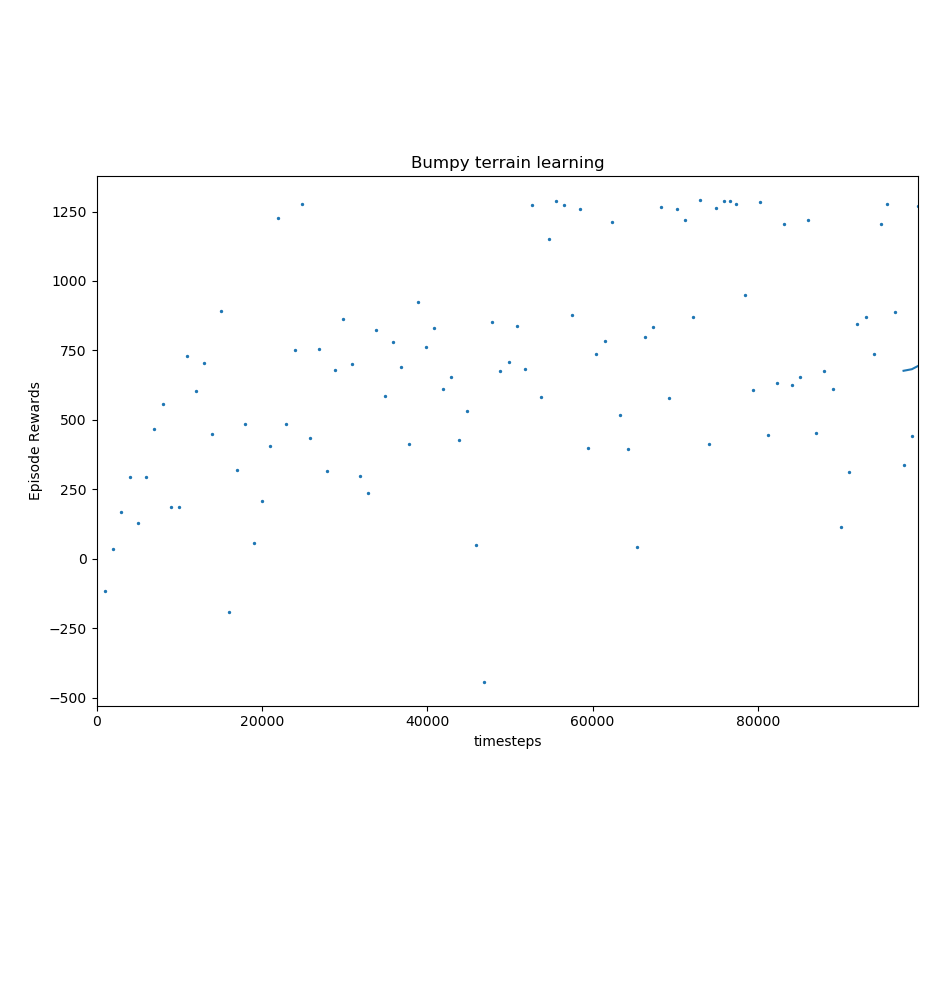
\includegraphics[width=.8\textwidth]{fig/Bumpy_terrain_learning_100ep_a2c.png}
% \end{figure}

\begin{figure}[ht]
\begin{subfigure}{.5\textwidth}
  \centering
  % include first image
  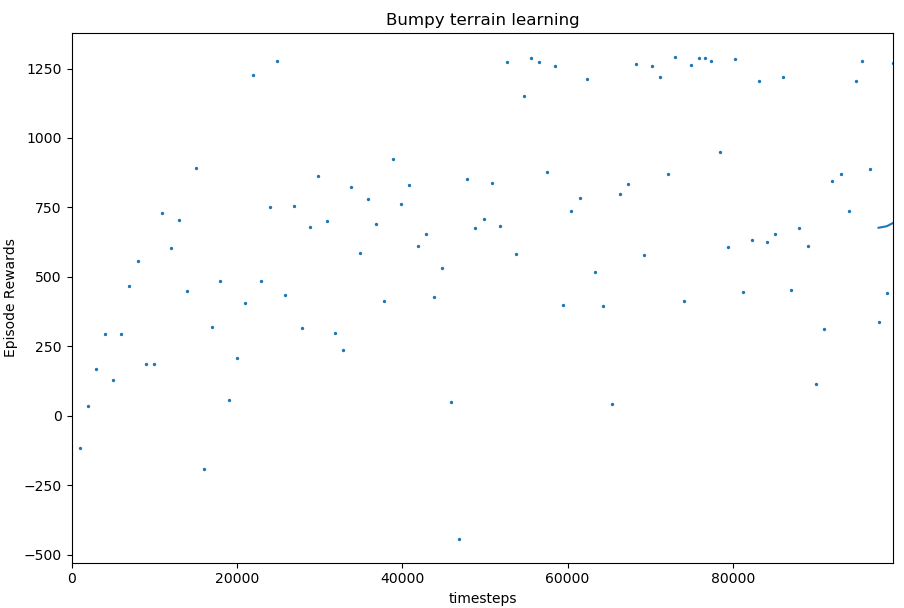
\includegraphics[width=.95\linewidth]{figc/Bumpy_terrain_learning_100ep_a2c.png}  
  \caption{A2C}
  \label{fig:sub-first}
\end{subfigure}
\begin{subfigure}{.5\textwidth}
  \centering
  % include second image
  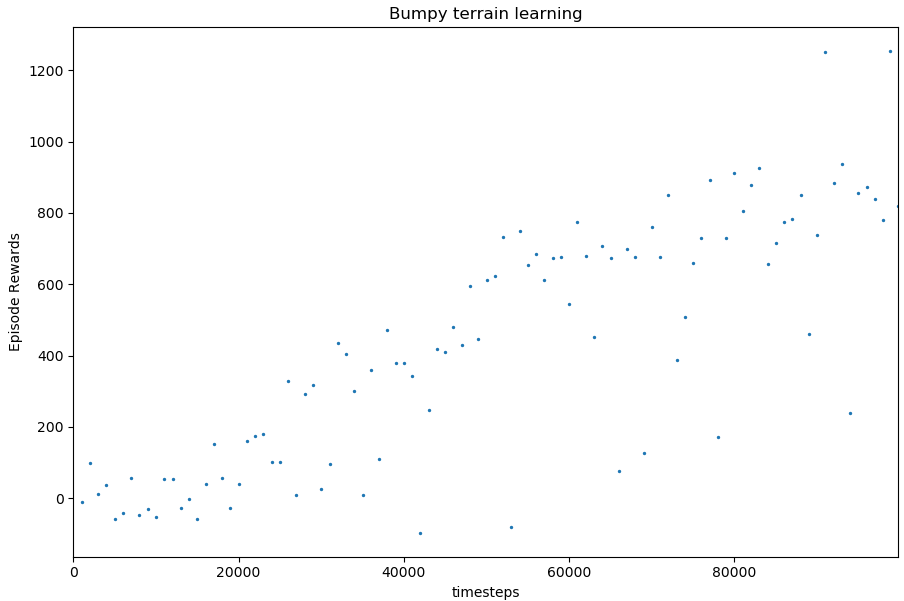
\includegraphics[width=.95\linewidth]{figc/Bumpy_terrain_learning_100ep_ppo.png}  
  \caption{PPO}
  \label{fig:sub-second}
\end{subfigure}
\caption{Put your caption here}
\label{fig:fig}
\end{figure}

\begin{figure}[ht]
\begin{subfigure}{.5\textwidth}
  \centering
  % include first image
  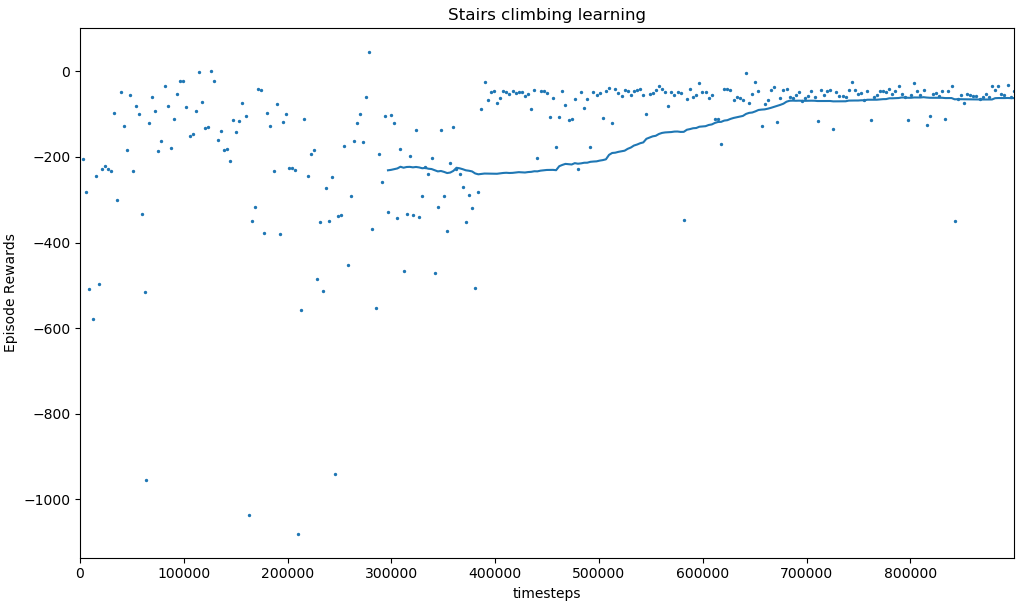
\includegraphics[width=.95\linewidth]{figc/Stairs_climbing_learning_300ep_final_a2c.png}  
  \caption{A2C}
  \label{fig:sub-first}
\end{subfigure}
\begin{subfigure}{.5\textwidth}
  \centering
  % include second image
  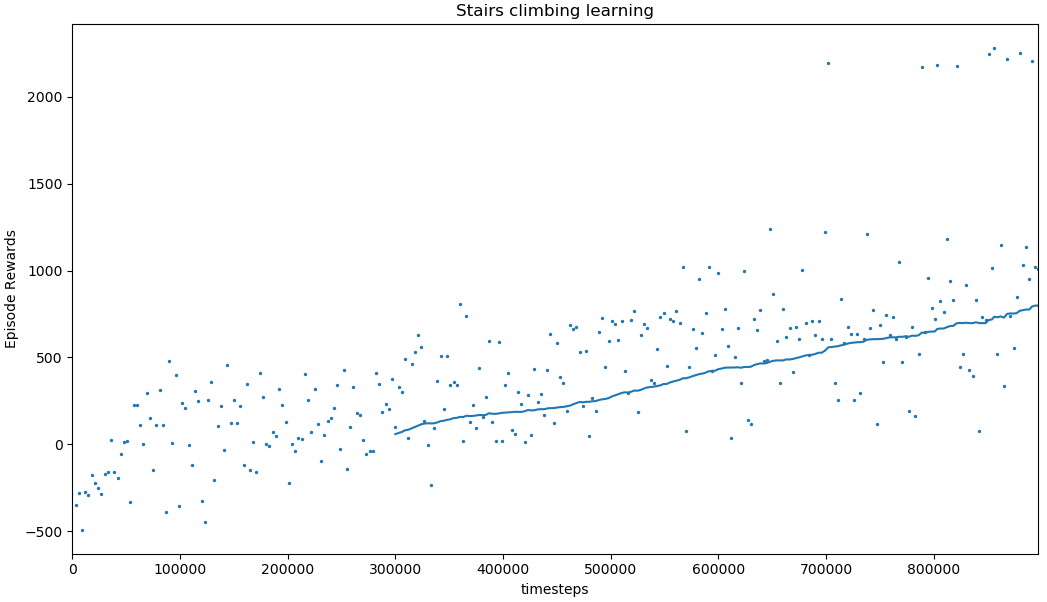
\includegraphics[width=.95\linewidth]{figc/Stairs_climbing_learning_300ep_final.png}  
  \caption{PPO}
  \label{fig:sub-second}
\end{subfigure}
\caption{Put your caption here}
\label{fig:fig}
\end{figure}

\cite{ppo}
VIDEO?
\section{Discussion}
Mention - happy that I was able to make it learn on the stairs and on the bumps.
Fun would be putting it on real HW and testing its movement and trying to bridge the reality gap (different masses, powers of motors, delays, springiness, ...) which would take a lot of effort, maybe for one full masters thesis.


% \bibliographystyle{IEEEtran}
\bibliographystyle{unsrt}
% DO NOT ERASE THE NEXT LINE,
% ONLY COMMENT IT AND DECOMMENT THE NEXT-NEXT, IF YOU NEED
% if you need it, get the repo git://redmine.laas.fr/laas/users/afranchi/bib.git and configure your bibinput in order to have : bibAlias,bibMain,bibNew,bibAF
% \bibliography{main.bib}
\bibliography{main.bib}

\end{document}
